\documentclass[twoside,a4paper,CCT]{cctart}   % 这是Li Dongfeng改的文件头
\usepackage{amsmath,amsthm,vatola,makeidx,amssymb,amscd,headrule}     % 这是Li Dongfeng改的文件头
\usepackage{amsfonts}                     % 这是Li Dongfeng改的文件头
%\documentstyle[twoside,headrule,vatola]{carticle} %这是原来的文件头
%\input amssym.def
\usepackage{graphicx}                              %这是原来的文件头
\usepackage{epsf}
\usepackage[top=1in,bottom=1in,left=1.25in,right=1.25in]{geometry}
\usepackage{amsmath}
\input scrload.tex    %调用花体字: {\scr A,B,C,...}
%--------------------------Page Format--------------------------
\headsep 0.2 true cm \topmargin 0pt \oddsidemargin 0pt \footskip
2mm \evensidemargin 0pt \textheight 21 true cm \textwidth 14.7
true cm \setcounter{page}{1}
%\parskip 0.2cm
\parindent 2\ccwd
\nofiles
%---------------------------------------------------------------
\def\sec#1{
\vskip.12in \noindent{\Large\bf\zihao{-4}\heiti #1} \vskip.1in}
\def\subsec#1{
\vskip.1in \flushpar{\zihao{5}\heiti #1} \vskip.1in}
\def\de#1{{\heiti\bf #1}\quad}

\begin{document}
\TagsOnRight \abovedisplayskip=10.0pt plus 2.0pt minus 2.0pt
\belowdisplayskip=10.0pt plus 2.0pt minus 2.0pt
%====================================================================
\catcode`@=11 \long\def\@makefntext#1{\parindent 1em\noindent
\hbox to 0pt{\hss$^{}$}#1} \catcode`\@=12
%====================================================================

\renewcommand{\baselinestretch}{1.0}


\newfont{\htxt}{eufm10 scaled \magstep0}
%\newfam\euffam
\font\tenthxt=eufm10 scaled \magstep0 \font\tenBbb=msbm10 scaled
\magstep0 \font\tencyr=wncyr10 scaled \magstep0 \font\tenrm=cmr10
scaled \magstep0 \font\tenbf=cmb10 scaled \magstep0


\def\cyr{\tencyr}
%\def\cyw{\eightcyr}
%\def\Bbb{\tenBbb}
%\def\bbb{\eightcyr}
%\def\txt{\tenthxt}

\def\ST{\songti\rm\relax}
\def\HT{\heiti\bf\relax}
\def\FS{\fangsong\relax}
\def\KS{\kaishu\relax}
\def\text#1{\hbox{\,#1\,}}
\def\pmb#1{\mbox{\boldmath $#1$}}
\def\Cal#1{{\cal #1}}

\def\CA{\Cal A}
\def\CB{\Cal B}
\def\cC{\Cal C}
\def\CD{\Cal D}
\def\CE{\Cal E}
\def\CF{\Cal F}
\def\CG{\Cal G}
\def\CH{\Cal H}
\def\CI{\Cal I}
\def\CJ{\Cal J}
\def\CK{\Cal K}
\def\CL{\Cal L}
\def\CM{\Cal M}
\def\CN{\Cal N}
\def\CO{\Cal O}
\def\CP{\Cal P}
\def\CQ{\Cal Q}
\def\CR{\Cal R}
\def\CS{\Cal S}
\def\CT{\Cal T}
\def\CU{\Cal U}
\def\CV{\Cal V}
\def\CW{\Cal W}
\def\CX{\Cal X}
\def\CY{\Cal Y}
\def\CZ{\Cal Z}
\def\BA {\hbox{\Bbb A}}
\def\BB {\hbox{\Bbb B}}
\def\BC {\hbox{\Bbb C}}
\def\BD {\hbox{\Bbb D}}
\def\BE {\hbox{\Bbb E}}
\def\BF {\hbox{\Bbb F}}
\def\BG {\hbox{\Bbb G}}
\def\BI {\hbox{\Bbb I}}
\def\BJ {\hbox{\Bbb J}}
\def\BK {\hbox{\Bbb K}}
\def\BL {\hbox{\Bbb L}}
\def\BM {\hbox{\Bbb M}}
\def\BN {\hbox{\Bbb N}}
\def\BO {\hbox{\Bbb O}}
\def\BP {\hbox{\Bbb P}}
\def\BQ {\hbox{\Bbb Q}}
\def\BR {\hbox{\Bbb R}}
\def\BS {\hbox{\Bbb S}}
\def\BT {\hbox{\Bbb T}}
\def\BU {\hbox{\Bbb U}}
\def\BV {\hbox{\Bbb V}}
\def\BW {\hbox{\Bbb W}}
\def\BX {\hbox{\Bbb X}}
\def\BY {\hbox{\Bbb Y}}
\def\BZ {\hbox{\Bbb Z}}
\def\Gh{\hbox{\htxt\char'150}}
\def\GG{\hbox{\htxt\char'107}}

\def\text#1{\hbox{\,#1\,}}
\def\pmb#1{\mbox{\boldmath $#1$}}
\def\Cal#1{{\cal #1}}

\newcommand{\orp}{\overline{\BR}_+}
\newcommand{\opm}{{\rm op}^{\frac{1}{2}-\delta}_M}
\newcommand{\wot}{\widehat{\otimes}_\pi}
\newtheorem{lemma}{引理}[section]
\newtheorem{guess}{猜测}[section]
\newtheorem{define}{定义}[section]
\newtheorem{theorem}{定理}[section]
%-----------------------作者定义


%-----------------------作者定义结束
\def\binom#1#2{{#1\choose#2}}
\def\qed{\hfill\raisebox{0.1truecm}{\framebox[0.2truecm]{\ } } }
\def\su{\mathop{\sum}\limits}
\def\Cal#1{ {\cal #1 \rm}  }
%---------------------------------------------------------------
\def\evenhead{{\protect\small{\zihao{-5}\songti \hfill \qquad\qquad
\qquad} \hfill {\zihao{-5}\songti }}}
\def\oddhead{{\protect\small {\zihao{-5}\songti }
\hfill {\small\zihao{-5}\songti }\hfill}}
%---------------------------------------------------------------

\vspace*{-13mm}

\thispagestyle{empty}

%%%%%%%%%%%%%%%%%%%%%%%%%%%%%%%%%%%%%%%%%%%%%%%%%%%%%%%%%%%%%%%%%


\ziju{0.025} \vspace*{.26in}

\centerline{\heiti\bf\zihao{2} $1X4$骨牌覆盖方形栅格的计数表示} \vskip .1in

%-------------------------------------------------------------------------

 %\footnotetext{基金项目: 国家自然科学基金资助课题(No. 10271026),
%福建省自然科学基金资助项目(No. F0310010).}

\footnotetext{E-mail: $*$ huih1984@163.com}

%-------------------------------------------------------------------------

\centerline{\fangsong\large\zihao{4} 惠慧$^{1}$ } \vskip.12in


\centerline{\small\zihao{-5}(1.南京大学数学系,南京,江苏, 210093)}

\vskip.25in

{\narrower\fangsong\zihao{-5}\small {\zihao{-5}\heiti 摘要:}\ \
在文章Kasteleyn$^{[1]}$中,Kasteleyn开创性研究了1X2骨牌在栅格上的覆盖数计算问题。那么如果是1X3骨牌或者1X4骨牌甚至更多,结果又是怎样的呢?文章忽略1X3骨牌的讨论,而直接讨论1X4骨牌的情况,因为从方法上可以是相似推广,可以沿用$Kasteleyn^{[1]}$ 中的方法。文章对内维数为2的情形$det(A)=pfaffian^{2}(A)$的结果做了推广,得出本文的一个关键结果即在内维数为4的情况下,定义矩阵和行列式以及$pfaffian$,得到$det(A)=pfaffian^{4}(A)$,最后着重讨论矩阵的计算问题。

{\zihao{-5}\heiti\tenbf 关键词:}\ \ 双重维数矩阵; 内维数; 多米诺覆盖; 外积; pfaffian; 1X2骨牌; 1X3骨牌; 1X4骨牌;

%{\tenbf\zihao{-5}\heiti MR(2000) 主题分类:}\ \ 54C10; 54D55 /
%{\tenbf\zihao{-5}\heiti 中图分类号:} O189.1


 }

\normalsize

\baselineskip 15pt \vskip.15in


\sec{0 引言}
数学公式在推广到更高阶的情形,情况往往变得复杂,比如方程解的问题,在小于五次时,有比较简单根式形式,而高于五次的方程一般而言没有根式解。理论的推广总是这样,去除局限的部分,余下的情形是可以扩张的!本文接下来就讨论1X4骨牌覆盖数的计算公式。

%很容易得到类似于$pfaffian$的表达形式,进而作者一直在寻找转换成矩阵表达形式,之所以这么做是因为从形式上来看,这种矩阵的存在完全符合数学符号的形式美,经过一番努力,终于找到了相应的矩阵形式。而这种拓展的矩阵形式本身却更有耐人寻味的结构美,作者没有见过有什么文献对这种形式的矩阵有深入的研究,这里作者只得出了一些少量的结果,作者能力有限,希望有更多的研究者参与其中来研究这种矩阵。

\sec{1 $1\times 4$覆盖数计数表示}


把问题转化成取每个小方块的端点,把一个$1\times 4$ tetramer转化为长为3的直线段。$C=(p_{1},p_{2},p_{3},p_{4})(p_{5},p_{6},p_{7},p_{8})...(p_{N-3},p_{N-2},p_{N-1},p_{N})$.\\
    其中$(p_{j},p_{j+1},p_{j+2},p_{j+3}),j=4k+1 (k=0,1,...)$为一个tetramer的四个连续点。为了一种覆盖对应于一种表示,要求满足

    \begin{equation}p_{1}<p_{2}<p_{3}<p_{4},p_{5}<p_{6}<p_{7}<p_{8}
   ,...,p_{N-3}<p_{N-2}<p_{N-1}<p_{N}\end{equation}

   \begin{equation}p_{1}<p_{5}<...<p_{N-3}\end{equation}

   这样的排列与$pfaffian$的排列不同,所以不再能用$pfaffian$来计算了。但是从形式上看这些排列与$pfaffian$要求的排列又很相似,只是
   作为一个小组的数字个数由2变成了4,
      \begin{equation}\sum\limits_{\sigma=p_{1}p_{2}...p_{N}satisfy(1)(2)}sgn\sigma a_{p_{1}p_{2}p_{3}p_{4}}a_{p_{5}p_{6}p_{7}p_{8}}...a_{p_{N-3}p_{N-2}p_{N-1}p_{N}}\end{equation}

   \begin{equation}a_{(i,j;i+1,j;i+2,j;i+3,j)}=1,1\leq i \leq m-3,1\leq j\leq n\end{equation}

   \begin{equation}a_{(i,j;i,j+1;i,j+2;i,j+3)}=(-1)^{i},1\leq i \leq m,1\leq j\leq n-3\end{equation}

   \begin{equation}a_{(i,j;i^{'},j^{'};i^{''},j^{''};i^{'''},j^{'''})}=0,other \end{equation}

   对应的矩阵记为$A_{4}=(a_{ijkl})$,满足$a_{jikl}=-a_{ijkl}$,$i,j,k,l$的任意一个序关系都满足逆序数正负号。
   这样得到的公式$(3)$,仍然称为$pfaffian(A_{4})$。从形式上讲,这样称呼完全正确!


从性质着手进行定义。
\sec{2 恒等式的证明}

{\bf 定义 1.1}\quad 双重维数矩阵
$\begin{bmatrix}
a_{i_{1}i_{2}...i_{n}}\end{bmatrix}_{m}$,$n$称为内维数,$m$称为外维数。

\newcounter{Lcount}
\begin{list}{\Roman{Lcount}}
{\usecounter{Lcount}
\setlength{\rightmargin}{\leftmargin}}
\tiny
\item
\begin{align*}
k det
  \begin{bmatrix}
  \begin{bmatrix}
 a_{1111}& a_{2111}&\cdots&a_{n111}\\
 a_{1211}& a_{2211}&\cdots&a_{n211}\\
 \cdots\\
a_{1n11}& a_{2n11}&\cdots&a_{nn11}\\
 \end{bmatrix}
\cdots
\begin{bmatrix}
a_{11n1}& a_{21n1}&\cdots&a_{n1n1}\\
a_{12n1}& a_{22n1}&\cdots&a_{n2n1}\\
 \cdots\\
a_{1nn1}& a_{2nn1}&\cdots&a_{nnn1}\\
\end{bmatrix}\\
\vdots\\
\begin{bmatrix}
a_{111n}& a_{211n}&\cdots&a_{n11n}\\
a_{121n}& a_{221n}&\cdots&a_{n21n}\\
\cdots\\
a_{1n1n}& a_{2n1n}&\cdots&a_{nn1n}\\
\end{bmatrix}
\cdots
\begin{bmatrix}
a_{11nn}& a_{21nn}&\cdots&a_{n1nn}\\
a_{12nn}& a_{22nn}&\cdots&a_{n2nn}\\
\cdots\\
a_{1nnn}& a_{2nnn}&\cdots&a_{nnnn}\\
\end{bmatrix}
\end{bmatrix}\\
\\
=det
  \begin{bmatrix}
  \begin{bmatrix}
 ka_{1111}& ka_{2111}&\cdots&ka_{n111}\\
 ka_{1211}& ka_{2211}&\cdots&ka_{n211}\\
 \cdots\\
ka_{1n11}& ka_{2n11}&\cdots&ka_{nn11}\\
 \end{bmatrix}
\cdots
\begin{bmatrix}
ka_{11n1}& ka_{21n1}&\cdots&ka_{n1n1}\\
ka_{12n1}& ka_{22n1}&\cdots&ka_{n2n1}\\
 \cdots\\
ka_{1nn1}& ka_{2nn1}&\cdots&ka_{nnn1}\\
\end{bmatrix}\\
\vdots\\
\begin{bmatrix}
a_{111n}& a_{211n}&\cdots&a_{n11n}\\
a_{121n}& a_{221n}&\cdots&a_{n21n}\\
\cdots\\
a_{1n1n}& a_{2n1n}&\cdots&a_{nn1n}\\
\end{bmatrix}
\cdots
\begin{bmatrix}
a_{11nn}& a_{21nn}&\cdots&a_{n1nn}\\
a_{12nn}& a_{22nn}&\cdots&a_{n2nn}\\
\cdots\\
a_{1nnn}& a_{2nnn}&\cdots&a_{nnnn}\\
\end{bmatrix}
\end{bmatrix}
 \end{align*}
 同样,对其它指标也成立。
 \item
\begin{align*}
det
  \begin{bmatrix}
\vdots\\
 \begin{bmatrix}
 a_{111i}& a_{211i}&\cdots&a_{n11i}\\
 a_{121i}& a_{221i}&\cdots&a_{n21i}\\
 \cdots\\
a_{1n1i}& a_{2n1i}&\cdots&a_{nn1i}\\
\end{bmatrix}
\cdots
\begin{bmatrix}
  a_{11ni}& a_{21ni}&\cdots&a_{n1ni}\\
  a_{12ni}& a_{22ni}&\cdots&a_{n2ni}\\
 \cdots\\
 a_{1nni}& a_{2nni}&\cdots&a_{nnni}\\
 \end{bmatrix}\\
\vdots\\
\begin{bmatrix}
  a_{111j}& a_{211j}&\cdots&a_{n11j}\\
  a_{121j}& a_{221j}&\cdots&a_{n21j}\\
   \cdots\\
   a_{1n1j}& a_{2n1j}&\cdots&a_{nn1j}\\
   \end{bmatrix}
\cdots
\begin{bmatrix}
  a_{11nj}& a_{21nj}&\cdots&a_{n1nj}\\
  a_{12nj}& a_{22nj}&\cdots&a_{n2nj}\\
   \cdots\\
   a_{1nnj }& a_{2nnj}&\cdots&a_{nnnj}\\
   \end{bmatrix}\\
\vdots\\
    \end{bmatrix}\\
=-det
  \begin{bmatrix}
\vdots\\
 \begin{bmatrix}
   a_{111j}& a_{211j}&\cdots&a_{n11j}\\
   a_{121j}& a_{221j}&\cdots&a_{n21j}\\
    \cdots\\
   a_{1n1j}& a_{2n1j}&\cdots&a_{nn1j}\\
   \end{bmatrix}
\cdots
\begin{bmatrix}
  a_{11nj}& a_{21nj}&\cdots&a_{n1nj}\\
  a_{12nj}& a_{22nj}&\cdots&a_{n2nj}\\
  \cdots\\
  a_{1nnj }& a_{2nnj}&\cdots&a_{nnnj}\\
  \end{bmatrix}\\
\vdots\\
 \begin{bmatrix}
   a_{111i}& a_{211i}&\cdots&a_{n11i}\\
   a_{121i}& a_{221i}&\cdots&a_{n21i}\\
 \cdots\\
a_{1n1i}& a_{2n1i}&\cdots&a_{nn1i}\\
\end{bmatrix}
\cdots
\begin{bmatrix}
  a_{11ni}& a_{21ni}&\cdots&a_{n1ni}\\
  a_{12ni}& a_{22ni}&\cdots&a_{n2ni}\\
 \cdots\\
  a_{1nni}& a_{2nni}&\cdots&a_{nnni}\\
  \end{bmatrix}\\
\vdots\\
    \end{bmatrix}
\end{align*}
 其它下标的任意两列交换,类似的符号变号。
 \item
\begin{align*}
det
  \begin{bmatrix}
\vdots\\
 \begin{bmatrix}
 a_{111i}& a_{211i}&\cdots&a_{n11i}\\
 a_{121i}& a_{221i}&\cdots&a_{n21i}\\
 \cdots\\
a_{1n1i}& a_{2n1i}&\cdots&a_{nn1i}\\
\end{bmatrix}
\cdots
\begin{bmatrix}
  a_{11ni}& a_{21ni}&\cdots&a_{n1ni}\\
  a_{12ni}& a_{22ni}&\cdots&a_{n2ni}\\
 \cdots\\
 a_{1nni}& a_{2nni}&\cdots&a_{nnni}\\
 \end{bmatrix}\\
\vdots\\
\begin{bmatrix}
  a_{111i}& a_{211i}&\cdots&a_{n11i}\\
  a_{121i}& a_{221i}&\cdots&a_{n21i}\\
   \cdots\\
   a_{1n1i}& a_{2n1i}&\cdots&a_{nn1i}\\
   \end{bmatrix}
\cdots
\begin{bmatrix}
  a_{11ni}& a_{21ni}&\cdots&a_{n1ni}\\
  a_{12ni}& a_{22ni}&\cdots&a_{n2ni}\\
   \cdots\\
   a_{1nni }& a_{2nni}&\cdots&a_{nnni}\\
   \end{bmatrix}\\
\vdots\\
    \end{bmatrix}\\
=0\\
\end{align*}

 \item
\begin{align*}
 det\begin{bmatrix}
 \begin{bmatrix}\begin{smallmatrix}
 a_{1111} + a_{1111}^{'}& a_{2111} + a_{2111}^{'}&\cdots&a_{n111} + a_{n111}^{'}\\
 a_{1211} + a_{1211}^{'}& a_{2211} + a_{2211}^{'}&\cdots&a_{n211} + a_{n211}^{'}\\
 \cdots\\
a_{1n11} + a_{1n11}^{'}& a_{2n11} + a_{2n11}^{'}&\cdots&a_{nn11} + a_{nn11}^{'}\\
\end{smallmatrix}\end{bmatrix}
\cdots
\begin{bmatrix}\begin{smallmatrix}
  a_{11n1} + a_{11n1}^{'}& a_{21n1} + a_{21n1}^{'}&\cdots&a_{n1n1} + a_{n1n1}^{'}\\
a_{12n1} + a_{12n1}^{'}& a_{22n1} + a_{22n1}^{'}&\cdots&a_{n2n1} + a_{n2n1}^{'}\\
 \cdots\\
 a_{1nn1} + a_{1nn1}^{'}& a_{2nn1} + a_{2nn1}^{'}&\cdots&a_{nnn1} + a_{nnn1}^{'}\\
 \end{smallmatrix}\end{bmatrix}\\
\vdots\\
\begin{bmatrix}
  a_{111n}& a_{211n}&\cdots&a_{n11n}\\
  a_{121n}& a_{221n}&\cdots&a_{n21n}\\
  \cdots\\
  a_{1n1n}& a_{2n1n}&\cdots&a_{nn1n}\\
  \end{bmatrix}
\cdots
\begin{bmatrix}
  a_{11nn}& a_{21nn}&\cdots&a_{n1nn}\\
  a_{12nn}& a_{22nn}&\cdots&a_{n2nn}\\
   \cdots\\
   a_{1nnn}& a_{2nnn}&\cdots&a_{nnnn}\\
\end{bmatrix}
\end{bmatrix}\\
\\
=det\begin{bmatrix}
 \begin{bmatrix}
   a_{1111}& a_{2111}&\cdots&a_{n111}\\
   a_{1211}& a_{2211}&\cdots&a_{n211}\\
 \cdots\\
a_{1n11}& a_{2n11}&\cdots&a_{nn11}\\
\end{bmatrix}
\cdots
\begin{bmatrix}
  a_{11n1}& a_{21n1}&\cdots&a_{n1n1}\\
  a_{12n1}& a_{22n1}&\cdots&a_{n2n1}\\
 \cdots\\
 a_{1nn1}& a_{2nn1}&\cdots&a_{nnn1}\\
 \end{bmatrix}\\
\vdots\\
\begin{bmatrix}
  a_{111n}& a_{211n}&\cdots&a_{n11n}\\
  a_{121n}& a_{221n}&\cdots&a_{n21n}\\
   \cdots\\
   a_{1n1n}& a_{2n1n}&\cdots&a_{nn1n}\\
   \end{bmatrix}
\cdots
\begin{bmatrix}
  a_{11nn}& a_{21nn}&\cdots&a_{n1nn}\\
  a_{12nn}& a_{22nn}&\cdots&a_{n2nn}\\
   \cdots\\
   a_{1nnn}& a_{2nnn}&\cdots&a_{nnnn}\\
   \end{bmatrix}
    \end{bmatrix}
  \\+det
  \begin{bmatrix}
 \begin{bmatrix}
   a_{1111}^{'}& a_{2111}^{'}&\cdots&a_{n111}^{'}\\
   a_{1211}^{'}& a_{2211}^{'}&\cdots&a_{n211}^{'}\\
 \cdots\\
a_{1n11}^{'}& a_{2n11}^{'}&\cdots&a_{nn11}^{'}\\
\end{bmatrix}
\cdots
\begin{bmatrix}
  a_{11n1}^{'}& a_{21n1}^{'}&\cdots&a_{n1n1}^{'}\\
  a_{12n1}^{'}& a_{22n1}^{'}&\cdots&a_{n2n1}^{'}\\
 \cdots\\
 a_{1nn1}^{'}& a_{2nn1}^{'}&\cdots&a_{nnn1}^{'}\\
 \end{bmatrix}\\
\vdots\\
\begin{bmatrix}
  a_{111n}& a_{211n}&\cdots&a_{n11n}\\
  a_{121n}& a_{221n}&\cdots&a_{n21n}\\
   \cdots\\
   a_{1n1n}& a_{2n1n}&\cdots&a_{nn1n}\\
   \end{bmatrix}
\cdots
\begin{bmatrix}
  a_{11nn}& a_{21nn}&\cdots&a_{n1nn}\\
  a_{12nn}& a_{22nn}&\cdots&a_{n2nn}\\
   \cdots\\
   a_{1nnn}& a_{2nnn}&\cdots&a_{nnnn}\\
   \end{bmatrix}
    \end{bmatrix}\\
    \end{align*}
   其它下标同样可以进行分拆。
   \item
$det \begin{bmatrix}
 \begin{bmatrix}
   1& 0&\cdots&0\\
   0& 0&\cdots&0\\
 \cdots\\
0& 0&\cdots&0\\
\end{bmatrix}
\cdots
\begin{bmatrix}
  0& 0&\cdots&0\\
  0& 0&\cdots&0\\
 \cdots\\
 0& 0&\cdots&0\\
 \end{bmatrix}\\
\vdots\\
\begin{bmatrix}
  0& 0&\cdots&0\\
  0& 0&\cdots&0\\
   \cdots\\
   0& 0&\cdots&0\\
   \end{bmatrix}
\cdots
\begin{bmatrix}
  0& 0&\cdots&0\\
  0& 0&\cdots&0\\
   \cdots\\
   0& 0&\cdots&1\\
   \end{bmatrix}
    \end{bmatrix}
    =1$
 \end{list}

\begin{theorem} 由上面的性质可以推导出双重维数矩阵的det
$$det(A_{4})=\sum \limits_{\sigma\tau\gamma}sgn\sigma sgn\tau sgn\gamma a_{\sigma(1)\tau(1)\gamma(1)1} a_{\sigma(2)\tau(2)\gamma(2)2}\cdots a_{\sigma(n)\tau(n)\gamma(n)n}$$
\end{theorem}
\begin{proof}
由$\textrm{IV}$ 得到左边等于
 \tiny \begin{equation}det\begin{bmatrix}
  \begin{bmatrix}
   a_{1111}& 0&\cdots&0\\
   0& 0&\cdots&0\\
 \cdots\\
0& 0&\cdots&0\\
\end{bmatrix}
\cdots
 \begin{bmatrix}
   0& 0&\cdots&0\\
   0& 0&\cdots&0\\
 \cdots\\
0& 0&\cdots&0\\
\end{bmatrix}\\
\vdots\\
\begin{bmatrix}
  a_{111n}& a_{211n}&\cdots&a_{n11n}\\
  a_{121n}& a_{221n}&\cdots&a_{n21n}\\
  \cdots\\
  a_{1n1n}& a_{2n1n}&\cdots&a_{nn1n}\\
  \end{bmatrix}
\cdots
\begin{bmatrix}
  a_{11nn}& a_{21nn}&\cdots&a_{n1nn}\\
  a_{12nn}& a_{22nn}&\cdots&a_{n2nn}\\
   \cdots\\
   a_{1nnn}& a_{2nnn}&\cdots&a_{nnnn}\\
\end{bmatrix}
\end{bmatrix}\end{equation}
$$+ \cdots\\$$
$$+
det\begin{bmatrix}
  \begin{bmatrix}
   0& 0&\cdots&0\\
   0& 0&\cdots&0\\
 \cdots\\
0& 0&\cdots&0\\
\end{bmatrix}
\cdots
 \begin{bmatrix}
   0& 0&\cdots&0\\
   0& 0&\cdots&0\\
 \cdots\\
0& 0&\cdots&a_{nnn1}\\
\end{bmatrix}\\
\vdots\\
\begin{bmatrix}
  a_{111n}& a_{211n}&\cdots&a_{n11n}\\
  a_{121n}& a_{221n}&\cdots&a_{n21n}\\
  \cdots\\
  a_{1n1n}& a_{2n1n}&\cdots&a_{nn1n}\\
  \end{bmatrix}
\cdots
\begin{bmatrix}
  a_{11nn}& a_{21nn}&\cdots&a_{n1nn}\\
  a_{12nn}& a_{22nn}&\cdots&a_{n2nn}\\
   \cdots\\
   a_{1nnn}& a_{2nnn}&\cdots&a_{nnnn}\\
\end{bmatrix}
\end{bmatrix}$$
对$(7)$式再进行分拆,由$I,V$得到
$det \begin{bmatrix}
 \begin{bmatrix}
   a_{1111}& 0&\cdots&0\\
   0& 0&\cdots&0\\
 \cdots\\
0& 0&\cdots&0\\
\end{bmatrix}
\cdots
\begin{bmatrix}
  0& 0&\cdots&0\\
  0& 0&\cdots&0\\
 \cdots\\
 0& 0&\cdots&0\\
 \end{bmatrix}\\
\vdots\\
\begin{bmatrix}
  0& 0&\cdots&0\\
  0& 0&\cdots&0\\
   \cdots\\
   0& 0&\cdots&0\\
   \end{bmatrix}
\cdots
\begin{bmatrix}
  0& 0&\cdots&0\\
  0& 0&\cdots&0\\
   \cdots\\
   0& 0&\cdots&a_{nnnn}\\
   \end{bmatrix}
   \end{bmatrix}
    =a_{1111}...a_{nnnn}$


    和一些其它项,诸如
    $sgn\sigma sgn\tau sgn\gamma  a_{1111}a_{2\sigma(2)\tau(2)\gamma(2)}...a_{n\sigma(n)\tau(n)\gamma(n)}$
    的项,可以由$I,II,V$得到。类似对其它项进行展开,即得结论。
\end{proof}

作为一个引申,也可以用外积来进行定义,
用外积来定义双重维数矩阵的行列式,
\begin{equation}
\begin{aligned}
\omega=
& \sum_{\substack{i_{\sigma}\in {(1,...,n)} j_{\sigma}\in {(1,...,n)}k_{\sigma}\in {(1,...,n)}l_{\sigma}\in{(1,...,n)}\\ i_{1} < i_{2} < i_{3} < i_{4}}}a_{i_{1}j_{1}k_{1}l_{1}}a_{i_{2}j_{2}k_{2}l_{2}}a_{i_{3}j_{3}k_{3}l_{3}}a_{i_{4}j_{4}k_{4}l_{4}}\\
& e_{1}^{i_{1}} \wedge e_{2}^{j_{1}} \wedge e_{3}^{k_{1}} \wedge e_{4}^{l_{1}} \wedge e_{1}^{i_{2}} \wedge e_{2}^{j_{2}} \wedge e_{3}^{k_{2}} \wedge e_{4}^{l_{2}} \wedge e_{1}^{i_{3}} \wedge e_{2}^{j_{3}} \wedge e_{3}^{k_{3}} \wedge e_{4}^{l_{3}} \wedge e_{1}^{i_{4}} \wedge e_{2}^{j_{4}} \wedge e_{3}^{k_{4}} \wedge e_{4}^{l_{4}}
\end{aligned}\end{equation}
\begin{equation}
\omega^{\frac{n}{4}}
\begin{aligned}
& = \frac{n}{4}! det(A) e_{1}^1\wedge e_{1}^2 \cdots \wedge e_{1}^n \wedge e_{2}^1\wedge e_{2}^2 \cdots \wedge e_{2}^n
\wedge e_{3}^1\wedge e_{3}^2 \cdots \wedge e_{3}^n \wedge e_{4}^1\wedge e_{4}^2 \cdots \wedge e_{4}^n
\end{aligned}\end{equation}

或者

\begin{equation}
\begin{aligned}
\omega_{i}=
& \sum_{j_{\sigma}\in {(1,...,n)}k_{\sigma}\in {(1,...,n)}l_{\sigma}\in{(1,...,n)}}a_{ij_{\sigma}k_{\sigma}l_{\sigma}} e_{1}^{j_{\sigma}} \wedge e_{2}^{k_{\sigma}} \wedge e_{3}^{l_{\sigma}}
\end{aligned}\end{equation}
\begin{equation}
\omega_{1}\wedge\omega_{2}\wedge\cdots\wedge\omega_{n}
\begin{aligned}
& = det(A) e_{1}^1\wedge e_{1}^2 \cdots \wedge e_{1}^n \wedge e_{2}^1\wedge e_{2}^2 \cdots \wedge e_{2}^n
\wedge e_{3}^1\wedge e_{3}^2 \cdots \wedge e_{3}^n
\end{aligned}
\end{equation}
从这里可以看出$det(A)$的几何意义,他是外积子空间做外积运算的一个度量。

pfaffian用外积来定义,
\begin{equation}\delta=\sum_{i<j<k<l}a_{ijkl}e^{i} \wedge e^{j} \wedge e^{k} \wedge e^{l}\end{equation}
\begin{equation}\delta^{\frac{n}{4}} = \frac{n}{4}! \operatorname{pf}(A)\;e^1\wedge e^2\wedge\cdots\wedge e^{n}\end{equation}

\begin{theorem}
矩阵$A_{4}$的下角标写成列向量形式,这里将列向量还是按照(1)(2)式的定义来定义了,实际上这不影响结论,只是记法上的差别。如果只有$$\begin{pmatrix}i\\i+1\\i+2\\i+3 \end{pmatrix},\begin{pmatrix}i+1\\i+2\\i+3\\i \end{pmatrix},\begin{pmatrix}i+2\\i+3\\i\\i+1 \end{pmatrix},\begin{pmatrix}i+3\\i\\i+1\\i+2 \end{pmatrix}$$和$$\begin{pmatrix}i\\i+4k\\i+8k\\i+12k \end{pmatrix},\begin{pmatrix}i+4k\\i+8k\\i+12k\\i \end{pmatrix},\begin{pmatrix}i+8k\\i+12k\\i\\i+4k \end{pmatrix},\begin{pmatrix}i+12k\\i\\i+4k\\i+8k \end{pmatrix}$$ 存在, 其它都为0。那么$$det(A)=pfaffian(A)^{4}$$
\end{theorem}

\begin{proof}
首先证明右边元素都落入左边,再证明左边元素都落入右边,最后证明符号相等。\\
将行列式的和式单项$a_{\sigma(1)\tau(1)\gamma(1)1} a_{\sigma(2)\tau(2)\gamma(2)2}\cdots a_{\sigma(n)\tau(n)\gamma(n)n}$ 下角标拿出来,构成矩阵:
\begin{equation}\begin{bmatrix}\sigma(1)&\sigma(2)&...&\sigma(n)\\\tau(1)&\tau(2)&...&\tau(n)\\\gamma(1)&\gamma(2)&...&\gamma(n)\\
1&2&...&n\end{bmatrix}\end{equation}
考虑元素的下标,将下标作为列向量写成普通矩阵形式。\\
将右边和式单项的下角标写成矩阵形式\begin{equation}\begin{bmatrix}p_{1}&p_{5}&...&p_{N-3}\\p_{2}&p_{6}&...&p_{N-2}\\p_{3}&p_{7}&...&p_{N-1}\\p_{4}&p_{8}&...&p_{N}\\\end{bmatrix}\end{equation}
那么需要证明左边矩阵和右边矩阵的的四次方存在一一对应。\\
这里的矩阵都忽略列向量间的互换,视为无差别。\\\\
第一步的证明:
将$1,...,n$进行分组
\begin{equation}\{1+16ik+4j,4+4k+16ik+4j,3+8k+16ik+4j,2+12k+16ik+4j \mid i=0,1,...;j=0,1,...,k-1\}\end{equation}
\begin{equation}\{2+16ik+4j,1+4k+16ik+4j,4+8k+16ik+4j,3+12k+16ik+4j \mid i=0,1,...;j=0,1,...,k-1\}\end{equation}
\begin{equation}\{3+16ik+4j,2+4k+16ik+4j,1+8k+16ik+4j,4+12k+16ik+4j \mid i=0,1,...;j=0,1,...,k-1\}\end{equation}
\begin{equation}\{4+16ik+4j,3+4k+16ik+4j,2+8k+16ik+4j,1+12k+16ik+4j \mid i=0,1,...;j=0,1,...,k-1\}\end{equation}
$(15)$中的$4$行元素从上至下分别对应于分组$(16)(17)(18)(19)$,显然是恰当的。同样的对应于分组
$$(17)(18)(19)(16),(18)(19)(16)(17),(19)(16)(17)(18),$$也是恰当的。将四次方乘积中的和式单项分别对应于四种不同的分组,恰好就得到一个左边的矩阵元$(3)$。\\
第二步的证明:将$(14)$中的列向量分成四组,第一组的列元素从上至下分别从属于$(16)(17)(18)(19)$,依次二三四组从属于$(17)(18)(19)(16),(18)(19)(16)(17),(19)(16)(17)(18)$,那么这四组分别对应于一个形式$(15)$,从而左边元落入右边。\\
第三步的证明:将右边元素看成都是从初始元(即$\begin{bmatrix}a\\a+1\\a+2\\a+3 \end{bmatrix}$形式)变换过来的,变换的规则为每次只允许进行四个元竖起来,或者四个并行进行左右移动一格。即
$$\begin{bmatrix}i&(i+4k)&(i+8k)&(i+12k)\\
(i+1)&(i+1+4k)&(i+1+8k)&(i+1+12k)\\
i+2&(i+2+4k)&(i+2+8k)&(i+2+12k)\\
i+3&(i+3+4k)&(i+3+8k)&(i+3+12k)\\\end{bmatrix}$$
$$\rightarrow\begin{bmatrix}i&(i+1+12k)&(i+2+8k)&(i+3+4k)\\
(i+4k)&(i+1)&(i+2+12k)&(i+3+8k)\\
i+8k&(i+1+4k)&(i+2)&(i+3+12k)\\
i+12k&(i+1+8k)&(i+2+4k)&(i+3)\\\end{bmatrix}$$
$$\rightarrow\begin{bmatrix}i&(i+4k)&(i+8k)&(i+12k)&i+4\\
(i+1)&(i+1+4k)&(i+1+8k)&(i+1+12k)&i+4+4k\\
i+2&(i+2+4k)&(i+2+8k)&(i+2+12k)&i+4+8k\\
i+3&(i+3+4k)&(i+3+8k)&(i+3+12k)&i+4+12k\\\end{bmatrix}$$
$$\rightarrow\begin{bmatrix}i&(i+1+4k)&(i+1+8k)&(i+1+12k)\\
(i+4k)&(i+2+4k)&(i+2+8k)&(i+2+12k)\\
i+8k&(i+3+4k)&(i+3+8k)&(i+3+12k)\\
i+12k&(i+4+4k)&(i+4+8k)&(i+4+12k)\\\end{bmatrix}$$ 那么通过这样的变换最终就可以得到最终元,而每一步的变换都不会带来符号上的改变,所以最终符号也是相同的,且这里还都是正号,即证。
\end{proof}

证明中关于等式右边的式子举例如下:
\begin{figure}[htbp]
  \centering
  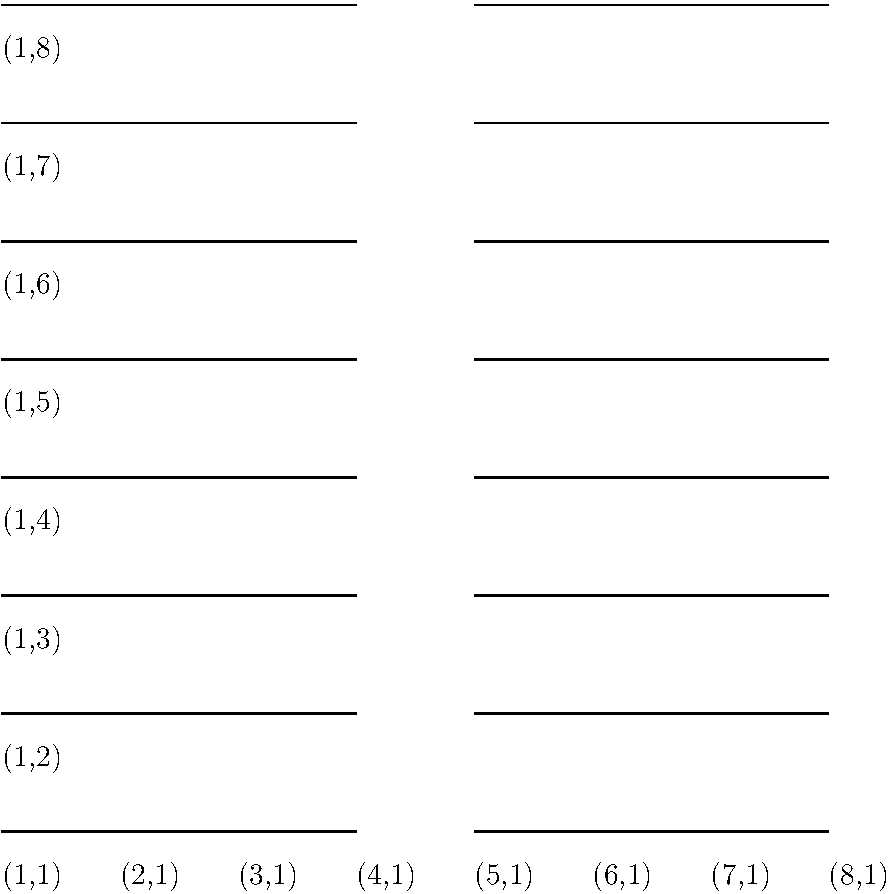
\includegraphics[width=0.35\textwidth]{c.pdf}
  \caption{Handwrite}\label{fig:digit}
\end{figure}
\begin{figure}[htbp]
  \centering
  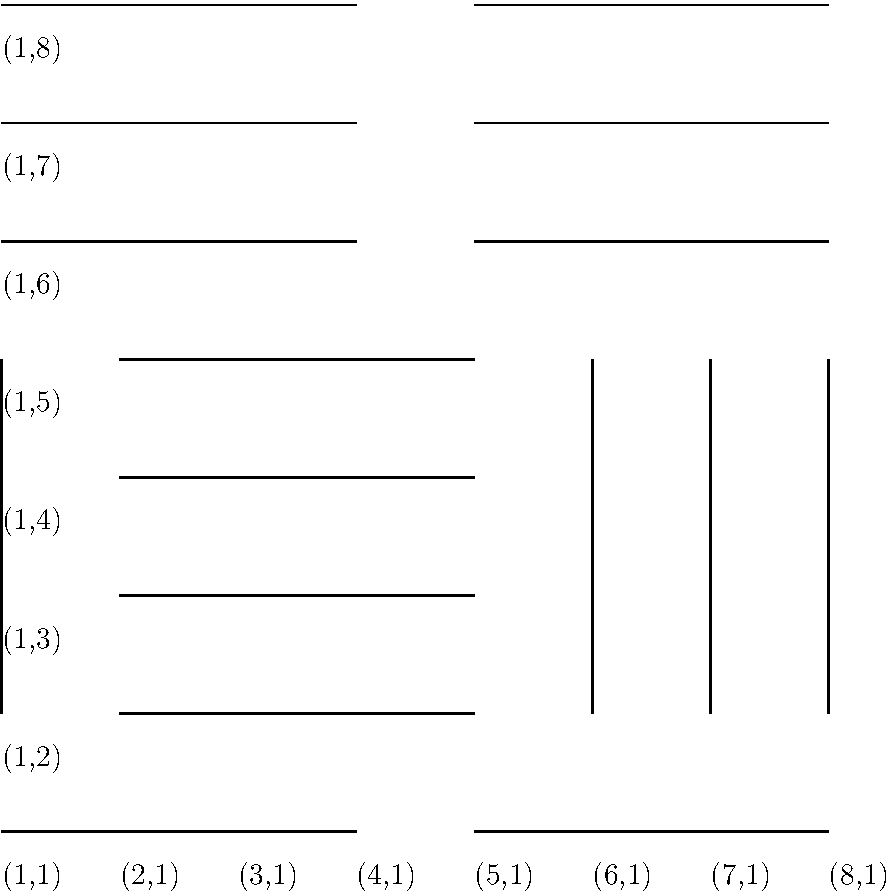
\includegraphics[width=0.35\textwidth]{d.pdf}
  \caption{Handwrite}\label{fig:digit}
\end{figure}\\
图1的矩阵
$$\begin{bmatrix}
1&5&12&16&19&23&26&30&33&37&44&48&51&55&58&62\\
2&6&9&13&20&24&27&31&34&38&41&45&52&56&59&63\\
3&7&10&14&17&21&28&32&35&39&42&46&49&53&60&64\\
4&8&11&15&18&22&25&29&36&40&43&47&50&54&57&61\\\end{bmatrix}$$
图2的矩阵
$$\begin{bmatrix}
1&5&33&12&19&26&37&30&23&16&44&48&51&55&58&62\\
2&6&9&13&20&27&34&38&31&24&41&45&52&56&59&63\\
3&7&17&10&21&28&35&14&39&32&42&46&49&53&60&64\\
4&8&25&11&18&29&36&22&15&40&43&47&50&54&57&61\\\end{bmatrix}$$

很容易验证这里举例的两个角标矩阵是满足证明中的第一步的分组性质的。
通过计算机编程,可以验证的结果如下:
方块为$1 \times 4$时,$det(A) = pfaffian(A)^{4} = 1$
方块为$4 \times4$时,$det(A) = pfaffian(A)^{4} = 16$
方块为$5 \times4$时,$det(A) = pfaffian(A)^{4} = 81$
\begin{theorem}
矩阵$A_{4}$的下角标写成列向量形式,如果每列元素只能是以4为周期的元素连续的顺序向量列之间行元素与行元素的交叉变换得到的列,其余都为0,那么仍然有$$det(A)=pfaffian(A)^{4}$$
\end{theorem}
\begin{proof}
归纳法。
首选对于矩阵外维数为4的情形显然成立,
假设在$4(n-1)$时成立,下证$4n$成立。
首先证明左边矩阵中的下标元矩阵都可以分解成四个pfaffian形式。假设存在某个列中包含$(4n-3,4n)$间的元素也包含$(1,4(n-1))$间的元素,
那么将这其中包含$(4n-3,4n)$间的元素剔除掉剩下的元素按某个周期归位,那么这个列上被$(4n-3,4n)$间元素所占据位置的元素,恰好都在某个$\xi$
列上,将这些元素还原,即可得到完全属于$(1,4(n-1))$之间的元素构成的列,而$\xi$变换得到的$\xi^{'}$如果还有元素$a$属于$(1,4(n-1))$间的元素,那么
肯定存在某个$\eta$中有元素属于这个元素$a$所在的周期,并且$\eta$中$a$元素所在的行位置恰好缺少的是$a$,我们先将$\eta$变换成只包含$a$所在周期的元素和$(4n-3,4n)$周期的元素$\eta^{'}$,基于假设,这总是可以做到的,那么交互$a$和$\eta^{'}$对应的行位置,那么得到的$\xi^{''}$最多还有一个元素不属于$(4n-3,4n)$周期,
如果确实还有一个这样的元素,类似的进行操作得到$\xi^{'''}$就是所有都在$(4n-3,4n)$周期的列了。类似的我们可以对其它列,其中包含$(4n-3,4n)$间的元素也包含$(1,4(n-1))$ 间的元素进行操作,最终得到完全属于$(4n-3,4n)$周期的列,因为对于每个列来说,列元素只能是以4为周期的顺序向量列之间行元素与行元素的交叉变换,所以这不会可之前的操作存在冲突,最终我们得到了四个元素都属于$(4n-3,4n)$间的列,和余下的列,那么有假设结论显然对变换后的这样的排列可以分解成四个pfaffian形式的列。
而变换都是可逆的,所以对于原始形式一样可以分解成四个pfaffian形式的列。四个右边可以合并成一个左边是显然的。
符号相同的证明,对于左边矩阵中的下标元矩阵由原始的正则型变换通过行变换而来,而每次变换都引起一次逆序数。这对于最终分斥的pfaffian形式来说也同样引起一次符号的变换,所以符号相同。
\end{proof}

\sec{3 计算}

{\bf 定义 1.4}\quad  双重维数矩阵的乘法
   $$[A_{ij}][B_{ijkl}]=[C_{ijkl}]$$
   $$c_{ijkl} = \Sigma_{\xi}^{n}a_{i\xi}b_{\xi jkl}$$

\begin{theorem}\quad  乘法定理

    $$det([A_{ij}][B_{ijkl}])=det([A_{ij}])det([B_{ijkl}])$$
\end{theorem}

{\bf 证明}\quad

\begin{align*}
det(C_{ijkl})&=\sum \limits_{\sigma\tau\gamma}sgn\sigma sgn\tau sgn\gamma c_{\sigma(1)\tau(1)\gamma(1)1} c_{\sigma(2)\tau(2)\gamma(2)2}\cdots c_{\sigma(n)\tau(n)\gamma(n)n}\\
&=\sum \limits_{\sigma\tau\gamma}sgn\sigma sgn\tau sgn\gamma \Sigma_{\xi}^{n}a_{\sigma(1)\xi}b_{\xi \tau(1)\gamma(1)1} \Sigma_{\xi}^{n}a_{\sigma(2)\xi}b_{\xi \tau(2)\gamma(2)2}\cdots \Sigma_{\xi}^{n}a_{\sigma(n)\xi}b_{\xi \tau(n)\gamma(n)n}\\
&=\sum \limits_{\tau\gamma}sgn\tau sgn\gamma(\sum \limits_{\sigma}sgn\sigma  \Sigma_{\xi}^{n}a_{\sigma(1)\xi}b_{\xi \tau(1)\gamma(1)1} \Sigma_{\xi}^{n}a_{\sigma(2)\xi}b_{\xi \tau(2)\gamma(2)2}\cdots \Sigma_{\xi}^{n}a_{\sigma(n)\xi}b_{\xi \tau(n)\gamma(n)n})\\
&=\sum \limits_{\tau\gamma}sgn\tau sgn\gamma(det([A_{ij}])\sum \limits_{\sigma}sgn\sigma b_{\sigma(1) \tau(1)\gamma(1)1} b_{\sigma(2) \tau(2)\gamma(2)1} \cdots b_{\sigma(n) \tau(n)\gamma(n)n})\\
&=det([A_{ij}])det([B_{ijkl}])
\end{align*}


或者通过外积形式证明如下:
令
$$(f_{1}^{1},f_{1}^{2},...,f_{1}^{n})=(e_{1}^{1},e_{1}^{2},...,e_{1}^{n})X_{1}$$
$$(f_{2}^{1},f_{2}^{2},...,f_{2}^{n})=(e_{2}^{1},e_{2}^{2},...,e_{2}^{n})X_{2}$$
$$(f_{3}^{1},f_{3}^{2},...,f_{3}^{n})=(e_{3}^{1},e_{3}^{2},...,e_{3}^{n})X_{3}$$
则
\begin{equation}
f_{1}^{j_{\sigma}}\wedge f_{2}^{k_{\sigma}}\wedge f_{3}^{l_{\sigma}}
\begin{aligned}
& = \sum_{\xi_{1}}\sum_{\xi_{2}}\sum_{\xi_{3}}x_{1}^{\xi_{1}j_{\sigma}}x_{2}^{\xi_{2}k_{\sigma}}x_{3}^{\xi_{
3}l_{\sigma}}e_{1}^{\xi_{1}}\wedge e_{2}^{\xi_{2}}\wedge e_{3}^{\xi_{3}}
\end{aligned}
\end{equation}

在$(f_{1}^{1},f_{1}^{2},...,f_{1}^{n}),(f_{2}^{1},f_{2}^{2},...,f_{2}^{n}),(f_{3}^{1},f_{3}^{2},...,f_{3}^{n})$
基底下的表示如下:
\begin{equation}
\begin{aligned}
\omega_{i}
&= \sum_{j_{\sigma}\in {(1,...,n)}k_{\sigma}\in {(1,...,n)}l_{\sigma}\in{(1,...,n)}}b_{ij_{\sigma}k_{\sigma}l_{\sigma}} f_{1}^{j_{\sigma}} \wedge f_{2}^{k_{\sigma}} \wedge f_{3}^{l_{\sigma}} \\
&= \sum_{j_{\sigma}\in {(1,...,n)}k_{\sigma}\in {(1,...,n)}l_{\sigma}\in{(1,...,n)}}b_{ij_{\sigma}k_{\sigma}l_{\sigma}}
\sum_{\xi_{1}}\sum_{\xi_{2}}\sum_{\xi_{3}}x_{1}^{\xi_{1}j_{\sigma}}x_{2}^{\xi_{2}k_{\sigma}}x_{3}^{\xi_{3}l_{\sigma}}e_{1}^{\xi_{1}}\wedge e_{2}^{\xi_{2}}\wedge e_{3}^{\xi_{3}}\\
&= \sum_{\xi_{1}}\sum_{\xi_{2}}\sum_{\xi_{3}}\sum_{j_{\sigma}\in {(1,...,n)}k_{\sigma}\in {(1,...,n)}l_{\sigma}\in{(1,...,n)}}b_{ij_{\sigma}k_{\sigma}l_{\sigma}}
x_{1}^{\xi_{1}j_{\sigma}}x_{2}^{\xi_{2}k_{\sigma}}x_{3}^{\xi_{3}l_{\sigma}}e_{1}^{\xi_{1}}\wedge e_{2}^{\xi_{2}}\wedge e_{3}^{\xi_{3}}
\end{aligned}\end{equation}
由此
$a_{ijkl}=\sum_{j_{\sigma}k_{\sigma}l_{\sigma}}b_{ij_{\sigma}k_{\sigma}l_{\sigma}}x_{1}^{jj_{\sigma}}x_{2}^{kk_{\sigma}}x_{3}^{ll_{\sigma}}$

\begin{equation}
\begin{aligned}
\omega_{1}\wedge\omega_{2}\wedge\cdots\wedge\omega_{n}
& = det(B) f_{1}^1\wedge f_{1}^2 \cdots \wedge f_{1}^n \wedge f_{2}^1\wedge f_{2}^2 \cdots \wedge f_{2}^n
\wedge f_{3}^1\wedge f_{3}^2 \cdots \wedge f_{3}^n\\
& = det(B)det(X_{1})det(X_{2})det(X_{3}) \\
&e_{1}^1\wedge e_{1}^2 \cdots \wedge e_{1}^n \wedge e_{2}^1\wedge e_{2}^2 \cdots \wedge e_{2}^n
\wedge e_{3}^1\wedge e_{3}^2 \cdots \wedge e_{3}^n\\
\end{aligned}
\end{equation}
由此得到$det(A) = det(B)det(X_{1})det(X_{2})det(X_{3})$
\\


\begin{theorem}  $A_{4}$的拉普拉斯定理
$$det(A)=\sum\limits_{j=1}^n \sum\limits_{k=1}^n \sum\limits_{l=1}^n (-1)^{i+j+k+l} a_{i,j,k,l} A_{i,j,k,l} $$
\end{theorem}
{\bf 证明}\quad
左边单项都属于右边且符号相同,项数也是相同的,结果是显而易见的。


推广的命题是,
$$detA=\sum\limits_{j_{1}j_{2}...j_{p}} \sum\limits_{k_{1}k_{2}...k_{p}} \sum\limits_{l_{1}l_{2}...l_{p}}
(-1)^{\sum_{t=1}^{p}(i_{t}+j_{t}+k_{t}+l_{t})}
M_{\left(\begin{array}{cccc}
i_{1} & i_{2} & \cdots & i_{p} \\
j_{1} & j_{2} & \cdots & j_{p} \\
k_{1} & k_{2} & \cdots & k_{p} \\
l_{1} & l_{2} & \cdots & l_{p} \\
\end{array}\right)}
A_{\left(\begin{array}{cccc}
i_{p+1} & i_{p+2} & \cdots & i_{n} \\
j_{p+1} & j_{p+2} & \cdots & j_{n} \\
k_{p+1} & k_{p+2} & \cdots & k_{n} \\
l_{p+1} & l_{p+2} & \cdots & l_{n} \\
\end{array}\right)}$$
项数上的关系是左边$(n!)^{3}$,右边是$(\frac{(n!)^{3}}{(p!(n-p)!))^{3}})(p!)^{3}[(n-p)!]^{3}$结论也比较显然。


\begin{define}
矩阵的叉积
\\
   $$\begin{bmatrix}\begin{smallmatrix}
  A_{11}& A_{12}& \cdots&A_{1n}\\
  A_{21}& A_{22}& \cdots&A_{2n}\\
  & & \cdots&\\&\\
  A_{n1}& A_{n2}& \cdots&A_{nn}\\
 \end{smallmatrix}\end{bmatrix}
 \times
 \begin{bmatrix}\begin{smallmatrix}
  B_{11}& B_{12}& \cdots&B_{1m}\\
  B_{21}& B_{22}& \cdots&B_{2m}\\
  & & \cdots&\\&\\
  B_{m1}& B_{m2}& \cdots&B_{mm}\\
 \end{smallmatrix}\end{bmatrix}\\$$
 $$=\\
 \begin{bmatrix}\begin{smallmatrix}
  A_{11} \times B_{11}& A_{12} \times B_{11}& \cdots&A_{1n} \times B_{11}
  & & \cdots&
  A_{11} \times B_{1m}& A_{12} \times B_{1m}& \cdots&A_{1n} \times B_{1m}\\
  A_{21} \times B_{11}& A_{22} \times B_{11}& \cdots&A_{2n} \times B_{11}
  & & \cdots&
  A_{21} \times B_{1m}& A_{22} \times B_{1m}& \cdots&A_{2n} \times B_{1m}\\
  & & & & &\cdots& &\\
  A_{n1} \times B_{11}& A_{n2} \times B_{11}& \cdots&A_{nn} \times B_{11}
  & & \cdots&
  A_{n1} \times B_{1m}& A_{n2} \times B_{1m}& \cdots&A_{nn} \times B_{1m}\\
  \cdots &\cdots &\cdots &\cdots &\cdots  &\cdots  &\cdots &\cdots  &\cdots &\cdots \\
  A_{11} \times B_{m1}& A_{12} \times B_{m1}& \cdots&A_{1n} \times B_{m1}
  & & \cdots&
  A_{11} \times B_{mm}& A_{12} \times B_{mm}& \cdots&A_{1n} \times B_{mm}\\
  A_{21} \times B_{m1}& A_{22} \times B_{m1}& \cdots&A_{2n} \times B_{m1}
  & & \cdots&
  A_{21} \times B_{mm}& A_{22} \times B_{mm}& \cdots&A_{2n} \times B_{mm}\\
  & & & & &\cdots& &\\
  A_{n1} \times B_{m1}& A_{n2} \times B_{m1}& \cdots&A_{nn} \times B_{m1}
  & & \cdots&
  A_{n1} \times B_{mm}& A_{n2} \times B_{mm}& \cdots&A_{nn} \times B_{mm}\\
  \end{smallmatrix}\end{bmatrix}$$
\end{define}


类似 Kasteleyn$^{[1]}$中将计算的矩阵表达成
$D=z(Q_{n}\times E_{m})  +  z^{'} (F_{n} \times Q_{m})$
由上面的定义,这里关于$tetramer$的计算也可以表达成两个类型的和式。
假设矩形方块为$n\times m$,
$$
  Q_{n} = \begin{bmatrix}\begin{smallmatrix}
  0& 0& 0&
  \begin{bmatrix}\begin{smallmatrix}
 0& 0& 0&0&\cdots&0\\
 0& 0& 0&0&\cdots&0\\
 0& 1& 0&0&\cdots&0\\
 0& 0& 0&0&\cdots&0\\
 & & \cdots& &\\
0& 0&0& 0&\cdots&0\\
 \end{smallmatrix}\end{bmatrix}& 0& 0& 0& \cdots&\\
 \begin{bmatrix}\begin{smallmatrix}
 0& 0& 0&0&\cdots&0\\
 0& 0& 0&0&\cdots&0\\
 0& 0& 0&0&\cdots&0\\
 0& 0& 1&0&\cdots&0\\
 & & \cdots& &\\
0& 0& 0& 0&\cdots&0\\
 \end{smallmatrix}\end{bmatrix}&
 0& 0& 0&
 \begin{bmatrix}\begin{smallmatrix}
 0& 0& 0&0&\cdots&0\\
 0& 0& 0&0&\cdots&0\\
 0& 0& 0&0&\cdots&0\\
 0& 0& 1&0&\cdots&0\\
 & & \cdots& &\\
0& 0& 0& 0&\cdots&0\\
 \end{smallmatrix}\end{bmatrix}&
 0& 0& \cdots&\\
 0& \begin{bmatrix}\begin{smallmatrix}
  0& 0& 0&0&\cdots&0\\
 0& 0& 0&0&\cdots&0\\
 0& 0& 0&0&\cdots&0\\
 0& 0& 0&0&\cdots&0\\
 0& 0& 0&1&\cdots&0\\
 & & \cdots& &\\
0& 0& 0& 0&\cdots&0\\
 \end{smallmatrix}\end{bmatrix}& 0& 0& 0&
 \begin{bmatrix}\begin{smallmatrix}
  0& 0& 0&0&\cdots&0\\
 0& 0& 0&0&\cdots&0\\
 0& 0& 0&0&\cdots&0\\
 0& 0& 0&0&\cdots&0\\
 0& 0& 0&1&\cdots&0\\
 & & \cdots& &\\
0& 0& 0& 0&\cdots&0\\
 \end{smallmatrix}\end{bmatrix}& 0& \cdots&\\
 0& 0& \ddots &0 &0 &0 &\ddots \\
\end{smallmatrix}\end{bmatrix}$$
$$= \begin{bmatrix}\begin{smallmatrix}
 0& 0& 0& A^{1}_{n} & 0 &\cdots& 0\\
 A^{2}_{n} & 0& 0& 0& A^{2}_{n} &\cdots& 0\\
 & & \cdots & &\\
 0& 0& 0& \cdots& 0& A^{n}_{n}& 0
\end{smallmatrix}\end{bmatrix}_{n} $$
$Q_{n}\times E_{m}$
那么有结果
$D=z(Q_{n}\times E_{m})  +  z^{'} (E_{n} \times Q_{m})$。\\

 \sec{参考文献}
\baselineskip 13pt {\footnotesize

\REF{[1]} P. W. Kasteleyn, The statistics of dimers on a lattice, {\it Physica.}, 1961, 27.

\REF{[2]} Richard Kenyon, Andrei Okounkov,  What is ... a dimer?, {\it Notices of the American Mathematical Society} MARCH 2005 VOLUME 52, NUMBER 3.

\REF{[3]} Henry Cohn, 2-adic behavior of domino tilings, {\it Electronic Journal of Combinatorics}, 6 1999.

\REF{[4]} Henry Cohn, Michael Larsen, James Propp, The shape of a typical boxed plane partition, {\it J of Math}, 1998.


\vskip .25in

\centerline{\Large\bf  The statistics of tetramers on a lattice }\vskip
.1in

\centerline{\normalsize\zihao{5} Hui Hui$^{1}$}\vskip .13in

{\small({\it  1. Department of Mathematics, NanJing University, Nanjing,
Jiangsu, 210093, P. R. China})}\vskip .23in

\baselineskip 14pt \zihao{5}\normalsize {\indent{\bf Abstract:}\ \
The article Kasteleyn$^{[1]}$ transfer dimer tiling to determinant of matrix ingenious, finally, get formula of it.
so, what about of three,four?this is intreseting.this article will written by author's thinking order.first discuss four
,and last three.and some geometric means will be discussed also.\\
{\bf Key words:double dimension matrix; inner dimension; domino tiling; wedge product; pfaffian;trimer; dimer; tertramer}\ \

}
\end{document}
